\chapter{Einleitung}
\section{Allgemeines}
Ein Audio-Bluetooth-Modul soll in einfacher Weise ein Audio-Signal von beispielsweise einem Smartphone ausgeben. Dabei ist eine hohe Kompatibilität mit viele Geräten wichtig, weil es sehr viele verschiedene Versionen von Bluetooth gibt. Da Bluetooth-Geräte meist abwärtskompatibel sind, ist es sinnvoll das Modul mit einer älteren BT-Version laufen zu lassen.

\section{Zielsetzung}
Es soll ein Print angefertigt werden auf dem sich das BT-Modul samt Versorgungsschaltung befindet. Auf diesem Print wird zusätzlich noch eine Additionsschaltung vorgesehen, um auch mit einem Klinkeneingang ein Signal zuführen zu können, falls das BT-Modul ausfällt.\\
Um eine leichtere Handhabung zu ermöglichen, muss auch ein Adapterprint für das BT-Modul angefertigt werden.

\section{Auswahl des Bluetooth-Moduls}
Wie bereits erwähnt soll das BT-Modul mit möglichst viele Geräten kompatibel sein, also mit einer älteren BT-Version laufen. Es sollte weiterhin eine möglichst einfache Bedienung für den Benutzer ermöglichen (beispielsweise Play-/Pausetaste).\\
Außerdem soll es bei geringen Kosten eine möglichst gute Verbindung, d.h. einen hohe Reichweite, erzielt werden.\\ \\
Nach ausführlicher Recherche wurde das Modul \enquote{XS3868 Revision 3} ausgewählt. Der darauf verbaute Chip \enquote{OVC3860} von \enquote{OmniVision Technologies} hat sich bereits in vielen anderen Projekten bewährt. 
%% Revision richtig?????

\chapter{Bluetooth-Modul XS3868}
\section{OVC3860}
In dem Chip ist außer der Bluetooth-Verbindung auch noch ein Stereo-Audio-Prozessor verbaut. Zusätzlich gibt es noch eine UART-Schnittstelle mithilfe man einige Einstellungen am Chip vornehmen kann. Eine kleine LiPo-Ladeschaltung ist ebenfalls vorhanden, wird aber in diesem Fall nicht verwendet.\\
Das Modul benötigt eine Versorgungsspannung von 3,3V bis 4,2V, wobei der Chip mit 1,8V versorgt wird. Diese Spannung wird auf dem Modul erzeugt.\\
Die verwendete BT-Version ist 2.0. Einige GPIO-Pins sind auf das Modul herausgeführt um Funktionen wie \enquote{Play/Pause} zu ermöglichen. Der Chip benötigt einen externen Speicher und eine Antenne (auf dem Modul) um ordnungsgemäß zu funktionieren.
\begin{figure} [h]
	\centering
	\caption{Blockschaltbild OVC3860}
	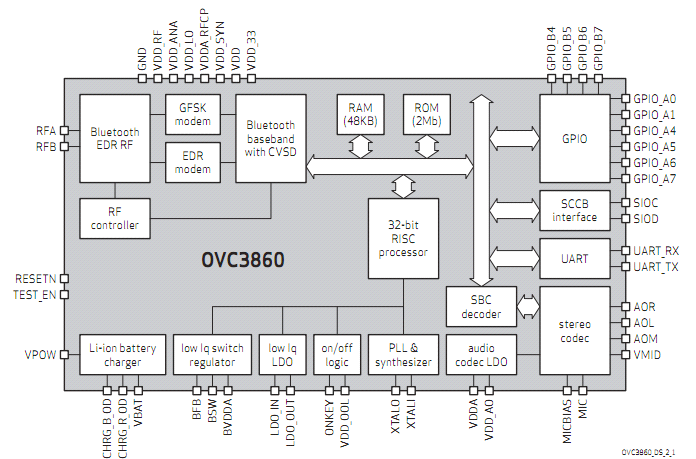
\includegraphics[width=0.8\textwidth]{img/blockschaltbild.png}
\end{figure}

\section{Pinbelegung}
Insgesamt hat das Modul 23 verwendbare Pins, aufgeteilt auf 2 Seiten in 11 und 12 Pins. 
\begin{figure} [h]
	\centering
	\caption{Pinbelegung XS3868}
	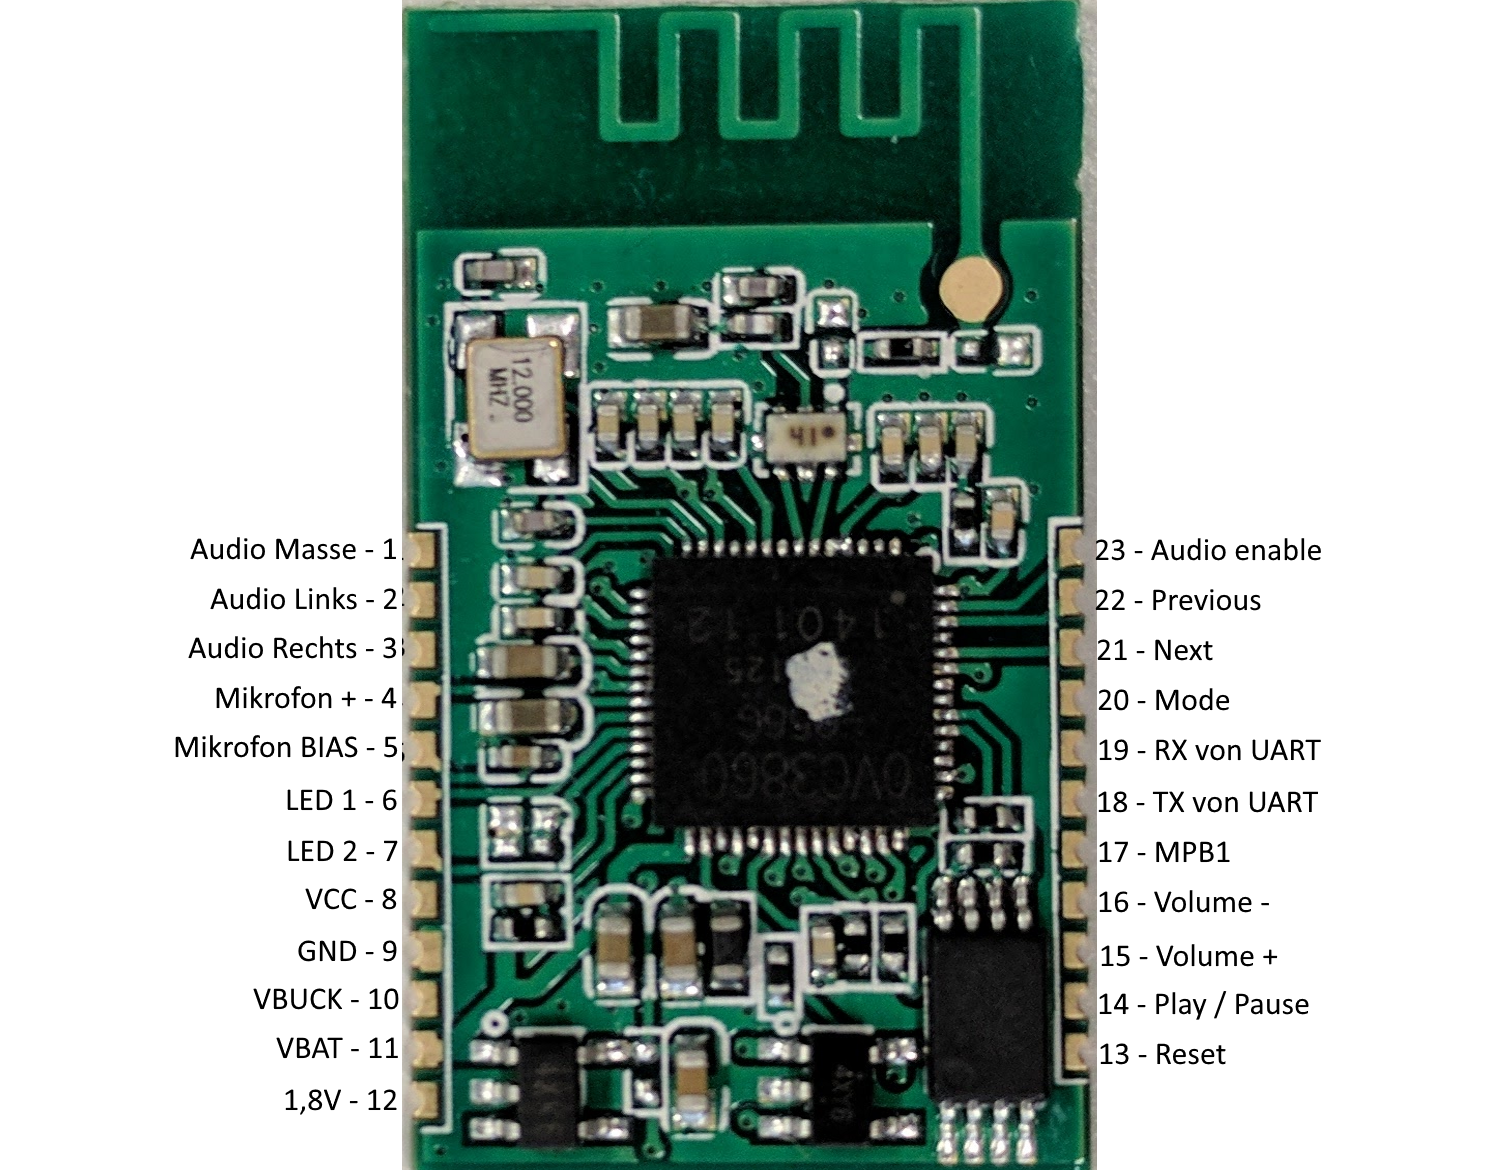
\includegraphics[width=1\textwidth]{img/XS3868_Pinbelegung.png}
\end{figure}\\
Wie in Abbildung 2.2 dargestellt, ist der Audio-Ausgang auf den Pins 1-3. Die Status-LED für das Modul wird mit dem Pin 6 geschaltet.\\
Die Versorgung des Moduls erfolgt über die Pins 11 (VBAT) und 9 (GND). Für die Audiofunktionen wird eine konstante Spannung (1,8V - Pin 12) benötigt. Diese Funktionen befinden sich auf den Pins 14-16 und 21-22. Sie werden mit Tastern beschalten.\\
Die UART-Schnittstelle befindet sich auf den Pins 18-19.\\
Außerdem verfügt das Modul auch über eine Mikrofon-Funktion, die aber in diesem Projekt nicht verwendet wird.

\section{Inbetriebnahme}
Bereits mit einer simplen Beschaltung kann das Modul in Betrieb genommen werden:
\begin{figure} [h]
	\centering
	\caption{Prinzipschaltung XS3868}
	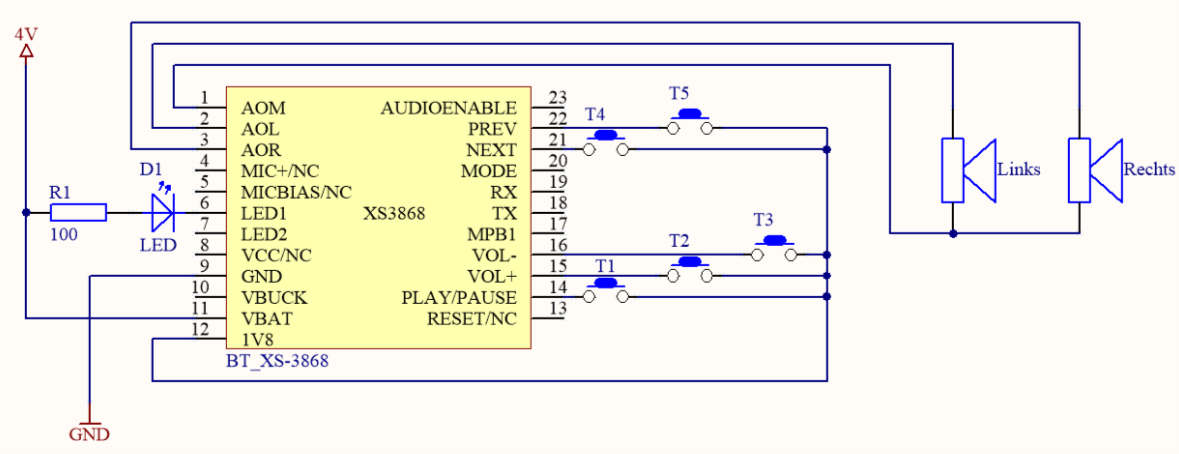
\includegraphics[width=1\textwidth]{img/XS3868_Prinzipschaltung}
\end{figure} \\
Mit dieser Schaltung kann das Modul bereits ordnungsgemäß arbeiten.\\
Die Status-LED ist, wie in Abbildung 2.3 dargestellt, \enquote{Low-Aktiv}. Beim Starten des Moduls und während der Suche nach Geräten blinkt sie durchgehend, wobei sie bei einer bestehenden Verbindung nur die Hälfte der Zeit blinkt.\\
Mit einfachem Betätigen eines Tasters wird die entsprechende Funktion vom Modul ausgeführt, jeweils mit einem Bestätigungston begleitet. Dieser Ton wird auch beim Starten des Moduls abgespielt.\\
Statt die Lautsprecher direkt an das Modul anzuschließen, sollte allerdings noch ein Verstärker verbaut werden.\\
Die Versorgungsspannung ist mit 4V etwas höher gewählt damit es nicht zu Ausfällen durch Spannungsschwankungen kommt. Das XS3868-Modul hat eine Stromaufnahme von ca. 30mA beim Starten, 10mA im Stand-By und bis zu 100mA wenn Musik abgespielt wird.

\section{Verbindung mit dem Modul}
Wenn der OVC3860 eingeschaltet ist, sucht er andauernd nach BT-Geräten. Er erscheint auf einem Smartphone so:

%% HIER FEHLT NOCH EIN BILD!!!!!







